\documentclass{article}
\usepackage[utf8]{inputenc}
\usepackage[margin=1in]{geometry}
\usepackage{amsmath, amsfonts}
\usepackage{fancyhdr}
\usepackage{multicol}
\usepackage{graphicx}
\usepackage[inline]{enumitem}
\graphicspath{ {images/} }
\pagestyle{empty}
\fancyhf{}
\cfoot{\thepage}
\pagenumbering{gobble}

\lhead{MATB42: Assignment \#6}
\rhead{
Poon, Keegan\\
1002423727\\
Mar 6th 2018}
\newcommand{\norm}[1]{\| #1 \|}
\newcommand{\deriv}[1]{\frac{d}{d #1}}
\newcommand{\parti}[1]{\frac{\partial}{\partial #1}}
\renewcommand{\headrulewidth}{0pt}
\newcommand{\gam}{\boldsymbol{\gamma}}
\begin{document}

\thispagestyle{fancy}

\begin{enumerate}
    \item Let $\displaystyle \omega = \frac{-y}{x^2+y^2}\ dx + \frac{x}{x^2+y^2}\ dy$. Calculate $\displaystyle \int_{\gam} \omega$ where
    \begin{enumerate}
        \item $\gam$ is the boundary of the triangle with vertices (in order) (0,1), (2,3) and (2,1).

        The triangle does not wrap around the origin, so the winding number is 0. This means the integral should also be 0
        \item $\gam$ is the boundary curve of the region $\displaystyle \Bigg\{(x,y) \in \mathbb{R}^2 \Bigg|\frac{(x-2)^2}{9} + \frac{(y+1)^2}{4} \leq 1 \Bigg\}$ oriented in a counter clockwise direction.

        This region is a disk and 0 satifies the equation, so the winding number of its surrounding ellipse is 1 (because the boundary curve is counter clockwise). This means the integral is $1(2\pi) = 2\pi$.
        \item $\gam$ is the graph of the polar equation $r = 3 + 2 \sin \theta$ oriented in the clockwise direction.

        Again, this curve wraps around the origin once, ($r > 0$ since $-2 \leq 2 \sin \theta \leq 2$), so the integral is $-2\pi$ since this wraps in the clockwise direction.
    \end{enumerate}
        \vspace{10ex}
    \item Let $\omega = (y^2 + z \ \ln 3)\ dx + (2xy + \sin z)\ dy + (y \cos z + (x + 1) \ln 3)\ dz$. Determine if $\omega$ is exact. If it is, use the algorithm given in class to find the potential function $g$.

        \begin{align*}
            &\frac{\partial F_1}{\partial y} = 2y & & \frac{\partial F_2}{\partial x} = 2y & & \frac{\partial F_3}{\partial x} = \ln 3& \\
            &\frac{\partial F_1}{\partial z} = \ln 3 & & \frac{\partial F_2}{\partial z} = \cos z & & \frac{\partial F_3}{\partial y} = \cos z& \\
        \end{align*}
        Since the pairwise differentials are equal, $\omega$ is closed. As well, the domain of polynomials and trig functions is $\mathbb{R}$ so the domain of $\omega$ is $\mathbb{R}^3$ which is simply connected $\implies \omega$ is exact. Given $F_1 = y^2 + z \ln 3$, $F_2 = 2xy + \sin z$, $F_3 = y \cos z + (x + 1) \ln 3$ where $\boldsymbol F = ( F_1,F_2, F_3 )$ then 
    \begin{align*}
        g &= \int F_1 dx = xy^2 + xz \ln 3 + f(y,z) \\
        F_2 &= \deriv{y} xy^2 + xz \ln 3 + f(y,z) \\
        2xy + \sin z &=  2xy + f'(y,z) \implies f(y,z) = y \sin z + f(z) \\
        F_3 &= \deriv{z} xy^2 + xz \ln 3 + y \sin z + f(z)\\
        y \cos z + (x + 1) \ln 3 &= x \ln 3 + y \cos z + f'(z) \implies f(z) = z \ln 3 + c \\
    \end{align*}
    This means that the potential function $g$ is $xy^2 + z(x+1)\ln 3+ y \sin z + c$
    \newpage
    \item Evaluate the double integral $\displaystyle \int_{-1}^{1} \int_{-\sqrt{1-x^2}}^{\sqrt{1-x^2}}3x^2y^2dy\ dx$, by first finding an equivalent line integral.

    Note that the region $R$ that is being integrated over is the unit circle in $\mathbb{R}^2$. We can parametrize the boundary of said circle using the path $\gam(t):[0,2\pi] \rightarrow \mathbb{R}^2$ by $t \mapsto (\cos t, \sin t )$. Using Green's theorem, choosing $F_2 = x^3y^2$ and $F_1 = 0$, we have:
    \begin{align*}
        \int_{-1}^{1} \int_{-\sqrt{1-x^2}}^{\sqrt{1-x^2}}3x^2y^2dy\ dx &= \int_{\gam} F_2dy = \int_0^{2\pi} \cos^3t \sin^2t ( \cos t)\ dt \\
        &= \int_0^{2\pi} \cos^4t \sin^2t\ dt = \frac{1}{4}\int_0^{2\pi}\cos^2 t(2 \sin t \cos t)^2 dt = \frac{1}{8}\int_0^{2\pi} (1 + \cos(2t))\sin^2 (2t) dt \\
        &\text{Let }u = \sin(2t), \: du = 2\cos(2t)dt \\
        &= \frac{1}{8}\Bigg[ \int_0^{2\pi} \sin^2(2t) dt +  \frac{1}{2}\int_0^{0}u^2du\Bigg] \\
        &= \frac{1}{16} \int_0^{2\pi} 1 - \cos(4t) dt \\
        &= \frac{\pi}{8}
    \end{align*}
\vspace{10ex}
    \item Let $R$ be a region in $\mathbb{R}^2$ and let $\gam$ be a counterclockwise parametrization of $\partial R$. Let $\boldsymbol F = (F_1,F_2)$ be a $C^1$ vector field defined throughout $R$ and on $\partial R$ and let $\boldsymbol n$ be the outward pointing unit normal vector to $\gam$. Use Green's theorem to give a double integral over $R$ which is equivalent to $\displaystyle \int_{\gam} \boldsymbol F \cdot \boldsymbol n \ ds$.

        Knowing that $\boldsymbol F \cdot \boldsymbol n = \norm{\boldsymbol F} \norm{\boldsymbol n} \cos \theta$ shows that no matter the actual direction of $\boldsymbol F$ and $\boldsymbol n$, as long as they are both angle $\theta$ away the dot product doesn't change. With this in mind, rotate $\boldsymbol F$ and $\boldsymbol n$ by $\frac{\pi}{2}$ so that we can get an expression for $\boldsymbol n$. Doing the rotation on $n$ will give a vector on the tangent, as it must be orthogonal, giving the expression $\frac{\gam ' (t)}{\norm{\gam ' (t)} }$ as it is unit length for the rotated $\boldsymbol n$ hereby referred to be $n'$. Given the expression for $\boldsymbol F$, it can be rotated with 
        \[F'= \begin{bmatrix} \cos \frac{\pi}{2} & -\sin \frac{\pi}{2} \\ \sin \frac{\pi}{2} & \cos \frac{\pi}{2} \end{bmatrix} \boldsymbol F = \begin{bmatrix} 0 & -1 \\ 1 & 0 \end{bmatrix} \begin{bmatrix} F_1 \\ F_2 \end{bmatrix} = (-F_2, F_1)\]
            Now the original integral can be rewritten as
        \begin{align*}
            &\int_{\gam}  F' \cdot n' \ ds& & =  \int_a^b  F'(\gam (t)) \cdot \frac{\gam ' (t)}{\norm{ \gam ' (t)} } \norm{\gam ' (t)}dt& \\
            && &= \int_a^b  F'(\gam (t)) \cdot \gam ' (t)dt &\\
            && &= \int_a^b -F_2dx + F_1 dy& \\
            && & =  \int_{\mathcal{R}} \frac{\partial F_1}{\partial x} + \frac{\partial F_2}{\partial y} dA & &\text{By Green's Theorem (Assuming $\gam$ is smooth)}&\\
        \end{align*}
    \newpage
    \item Give a parametrization for each of the following surfaces, use a computer algebra sustem to plot the surface and find a unit vector normal to the surface.
    \begin{enumerate}
        \item The piece of the cylinder $y^2 + z^2 = 1$ between $x = -1$ and $x = 3$.
        
        The cylinder can be parametrized as a circle in the y,z plane i.e. $y, z = (\cos \theta, \sin \theta)$. Restricting x gives 
            \[\boldsymbol \Phi (x, \theta) = (x, \cos \theta, \sin \theta)\]
            where $ -1 \leq x \leq 3$ and $0 \leq \theta \leq 2\pi$.
        
            To find a normal vector, first need to figure out the tangent vectors. $\boldsymbol \phi_x = (1,0,0), \boldsymbol \phi_{\theta} = (0, -\sin \theta, \cos \theta)$, so a normal vector is 
            \[\boldsymbol \phi_x \times \boldsymbol \phi_{\theta} = (0, -\cos \theta, - \sin \theta)\] The magnitude of said vector is already one, so it is a unit normal vector to the surface.

        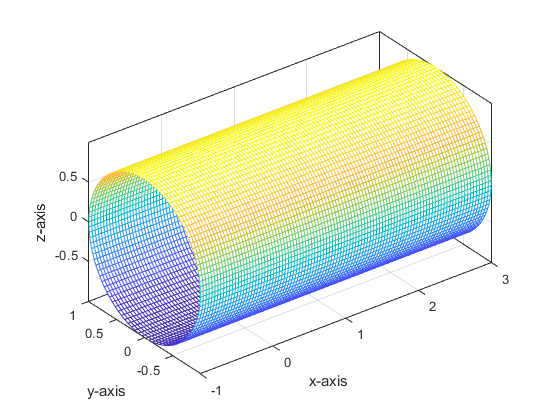
\includegraphics[width=\textwidth]{b42-a6-5a}

        \item The piece of the plane $z = x + y + 5$ which lies over the unit disk $x^2 + y^2 \leq 1$.
        
        Since working with a disk, switch to polar coordinates to describe the domain where $x, y = (r \cos \theta, r \sin \theta)$ having $0 \leq r \leq 1$ and $ 0 \leq \theta \leq 2\pi$.
            
            Now the surface can be parameterized by the given expression for $z$: \[\boldsymbol \Phi (r, \theta) = (r \cos \theta, r \sin \theta, r (\cos \theta + \sin \theta ) + 5)\] The tangent vectors of this plane are $\boldsymbol \phi_r = (\cos \theta, \sin \theta, \cos \theta + \sin \theta)$ and $\boldsymbol \phi_{\theta} = (-r\sin \theta, r\cos \theta, r(- \sin \theta + \cos \theta))$. The normal vector is therefore $\boldsymbol \phi_r \times \boldsymbol \phi_{\theta} = (\sin\theta r (\cos \theta - \sin \theta) - (\cos \theta + \sin \theta)r\cos \theta, (\cos \theta + \sin \theta)(-r\sin \theta) - (\cos \theta)r(\cos \theta - \sin \theta), \cos \theta (r\cos \theta) - \sin \theta (-r \sin \theta)) = (-r, -r, r)$. Dividing by the magnitude of the vector $\sqrt{3r^2} = \sqrt{3}r$ gives the unit vector \[\frac{1}{\sqrt{3}}(-1,-1,1)\]

        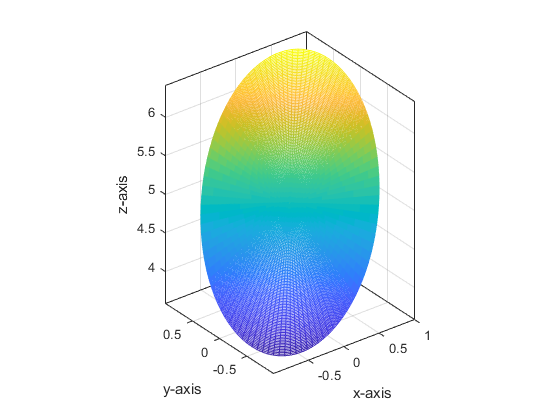
\includegraphics[width=\textwidth]{b42-a6-5b}

        \item The piece of the sphere $x^2 + y^2 + z^2 = 4$ which lies above the plane $z = 1$.

        The sphere can be parametrized in a standard way as $\boldsymbol \Phi (u,v) \mapsto (2 \cos u \sin v, 2 \sin u \sin v, 2 \cos v)$ To restrict this surface to only the portion that lies above $z = 1$, take the $z$ of the parametrization and restrict it. This gives $2 \cos v > 1 \implies \cos v > 1/2 \implies v < \arccos 1/2 = \pi/3$ since arccos strictly decreasing so $0 < v < \pi/3$. The other angle being restricted to $0 \leq u \leq 2\pi$. The tangent vectors to the plane are 
        \begin{align*}
            \boldsymbol \phi_u &= (-2\sin u \sin v, 2 \cos u \sin v, 0) \\
            \boldsymbol \phi_v &= (2 \cos u \cos v, 2 \sin u \cos v, -2 \sin v) \\
            \text{Now the normal vector is} \\
            \boldsymbol \phi_u \times \boldsymbol \phi_v &= (-4 \cos u \sin^2 v, -4 \sin u \sin ^2 v, -4 \sin^2 u \cos v \sin v -4 \cos^2 u \cos v \sin v) \\
            &= -4 (\cos u \sin^2 v, \sin u \sin ^2 v, \cos v \sin v) \\
            \text{The magnitude of which is} \\
            \norm{\boldsymbol \phi_u \times \boldsymbol \phi_v} &= 4 \sqrt{ \cos^2 u \sin ^ 4 v + \sin ^2 u \sin ^4 v + \cos ^2 v \sin ^2 v} \\
            &= 4 \sqrt{ (\cos^2 u + \sin ^2 u) \sin ^4 v + \cos ^2 v \sin ^2 v} \\
            &= 4 \sqrt{ (\sin^2 v + \cos ^2 v) \sin ^2 v} \\
            &= 4 | \sin v | \\
            \text{So the unit normal vector is}
            &= -\frac{1}{| \sin v |} (\cos u \sin^2 v, \sin u \sin ^2 v, \cos v \sin v) \\
        \end{align*}

        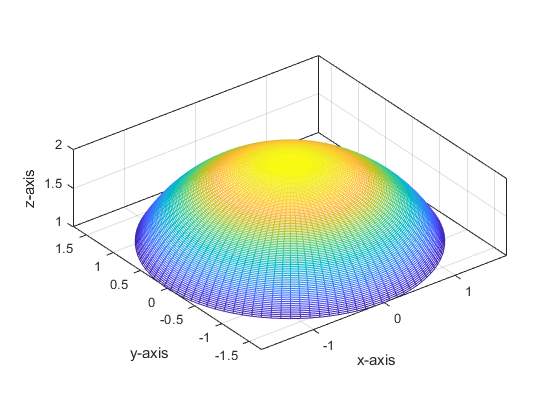
\includegraphics[width=\textwidth]{b42-a6-5c}

        \item The piece of the plane $x + y + z = 1$ which lies above the parallelogram: $0 \leq y - x \leq 1, 0 \leq y + 2x \leq 1$.
        
        Want to parametrize easier, so choose variables to exploit this, $u = y - x, v = y + 2x$
        \begin{align*}
            & 2u + v = 3y & &\implies& &y = \frac{2u + v}{3}& \\
            &v - u = 3x& &\implies& &x = \frac{v - u}{3}& \\
            &z = 1 - x - y& &\implies& &z = \frac{1}{3}(3 -v + u -2u -v) = \frac{3 -2v -u}{3}& \\
        \end{align*}
        So $\boldsymbol \Phi(u,v) \mapsto \frac{1}{3}(v - u, 2u + v, 3 - 2v -u)$ where $0 \leq u , v \leq 1$.
        Then the tangents are
        \begin{align*}
            \boldsymbol \phi_u &= \frac{1}{3}(-1, 2, -1) \\
            \boldsymbol \phi_v &= \frac{1}{3}(1,1,-2) \\
            \boldsymbol \phi_u \times \boldsymbol \phi_v &= \frac{1}{3}((2)(-2) - (-1)(1), (-1)(1) - (-1)(-2), (-1)(1) - (2)(1)) \\
            &= \frac{1}{3}(-4 + 1, -1 - 2, -1 - 2) = -(1,1,1)
        \end{align*}
            So the unit normal is $(\frac{1}{\sqrt{3}},\frac{1}{\sqrt{3}},\frac{1}{\sqrt{3}})$

        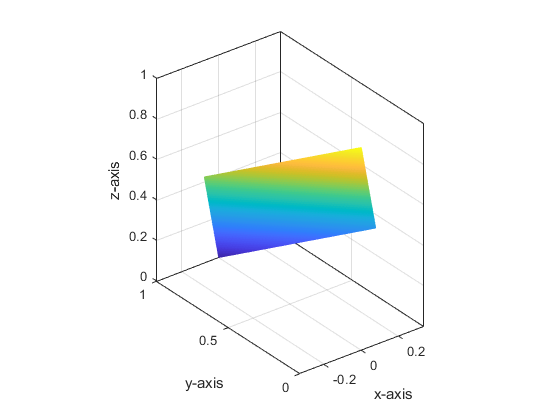
\includegraphics[width=\textwidth]{b42-a6-5d}
    \end{enumerate}
    \newpage
    \item Let $S$ be the surface given parameterically by $\boldsymbol \Phi (u,v) = (u^2, 3v, u^2 + v)$ where $(u,v) \in D$, the interior of a triangle with vertices (0,0), (3,0) and (3,3).
    \begin{enumerate}
        \item Find the surface area of $S$.
        \begin{align*}
            \boldsymbol \phi_u &= (2u, 0, 2u) \\
            \boldsymbol \phi_v &= (0, 3, 1) \\
            \boldsymbol \phi_u \times \boldsymbol \phi_v &= (0 - 6u, 0 - 2u, 6u - 0) = (-6u, -2u, 6u) \\
            \norm{\boldsymbol \phi_u \times \boldsymbol \phi_v} &= \sqrt{36u^2 + 4u^2 + 36u^2} = \sqrt{76}u \text{ u positive in the triangle}\\
            \int_D \norm{\boldsymbol \phi_u \times \boldsymbol \phi_v} dA &= \int_0^3\int_0^u \sqrt{76}u dv du = \int_0^3 \sqrt{76}{u^2} du = \frac{\sqrt{76}}{3}3^3 = 9\sqrt{76}        
        \end{align*}
        \item Find the equation of the tangent plane to $S$ at the point (4,9,7).
        
        The equation for the tangent plane is given by $(\boldsymbol \phi_u \times \boldsymbol \phi_v \cdot (4-x,9-y,7-z)) = 0$. We know that $\boldsymbol \Phi (u_0, v_0) = (4,9,7)$ so $u_0 = 2, v_0 = 3$. This means the normal vector is $(-12,-4,12) \implies$ the tangent plane is $(-12)(4-x) + (-4)(9-y) + (12)(7-z) = 0$.
        \[ \implies 12x + 4y - 12z = -36 \]
    \end{enumerate}
    \vspace{10ex}
    \item Suppose the surface $S$ is the graph of a function $f : \mathbb{R}^2 \rightarrow \mathbb{R}$. Give a natural parametrization of $S$ (in terms of $f$) and derive the formula $\norm{\boldsymbol \phi_u \times \boldsymbol \phi_v} = \sqrt{1 + \norm{\text{grad }f}^2}$

    The surface $S$ can be parametrized naturally as $\boldsymbol \Phi (u,v) = (u, v, f(u,v))$

    This means the tangent vectors can be written as
    \begin{align*}
        \boldsymbol \phi_u &= (1, 0, \frac{\partial}{\partial u} f(u,v)) \\
        \boldsymbol \phi_v &= (0, 1, \frac{\partial}{\partial v} f(u,v)) \\
        \boldsymbol \phi_u \times \boldsymbol \phi_v &= ( - \frac{\partial}{\partial u} f(u,v),  - \frac{\partial}{\partial v} f(u,v), 1) \\
        \norm{\boldsymbol \phi_u \times \boldsymbol \phi_v} &= \sqrt{(\frac{\partial}{\partial u} f(u,v))^2 + (\frac{\partial}{\partial v} f(u,v))^2 + 1} \\
        &= \sqrt{ (\frac{\partial}{\partial u} f(u,v), \frac{\partial}{\partial v} f(u,v)) \cdot (\frac{\partial}{\partial u} f(u,v), \frac{\partial}{\partial v} f(u,v)) + 1} \\
        &= \sqrt{\nabla f \cdot \nabla f + 1} \\
        &= \sqrt{\norm{\nabla f}^2 + 1} \\
    \end{align*}
    \newpage
    \item A paraboloid of revolution $S$ is parameterized by $\boldsymbol \Phi (u,v) = (u \cos v, u \sin v, u^2$), $0 \leq u \leq 2, 0 \leq v \leq 2\pi$.
    \begin{enumerate}
        \item Find an equation in $x,y$ and $z$ describing the surface.

        Looking at the first two elements of the surface, $u \cos v$ and $u \sin v$, $x^2 + y^2 = u^2 \cos^2 v + u^2 \sin ^2 v = u^2 = z^2$. So the equation is just $x^2 + y^2 = z^2$.
        \item What are the geometric meanings of the parameters $u$ and $v$?

        The $v$-curves are the rings of the paraboloid, at a given height level, while $u$-curves are the parabolas that stretch down the paraboloid vertically, so $v$ is the angle on the paraboloid, and $u$ is the height.
        \item Find a unit vector orthogonal to the surface of $\boldsymbol \Phi (u,v)$.
        \begin{align*}
            \boldsymbol \phi_u &= (\cos v, \sin v, 2u) \\
            \boldsymbol \phi_v &= (-u \sin v, u \cos v, 0) \\
            \boldsymbol \phi_u \times \boldsymbol \phi_v &= (-2u^2 \cos v, -2u^2 \sin v, u \cos^2 v + u \sin^2 v) \\
            &= u(-2u\cos v, -2u\sin v , 1) \\
            \norm{\boldsymbol \phi_u \times \boldsymbol \phi_v} &= u\sqrt{4u^2 \cos^2 v + 4u^2 \sin^2 v + 1} \\
            &= u\sqrt{4u^2 + 1} \\
            \text{Normal unit vector } \boldsymbol n(u,v) &= \frac{1}{\sqrt{4u^2 +1}}(-2u \cos v, -2u\sin v , 1) \\
        \end{align*}
        \item Find the equation for the tangent plane at $\boldsymbol \Phi(u_0,v_0) = (1,1,2)$ and express your answer in the following two ways:
        \begin{align*}
            u_0^2 = 2 \implies u_0 = \sqrt{2} \\
            \sqrt{2} \cos (v_0) = \sqrt{2} \sin (v_0) = 1 \\ 
            \implies \sin(v_0) = \cos(v_0) = \frac{1}{\sqrt{2}} \implies v_0 = \frac{\pi}{2}
        \end{align*} 
        \begin{enumerate}
            \item parameterized by $u$ and $v$; and
                \begin{align*}
                    \boldsymbol \phi_u(\sqrt2 , \frac{\pi}{2}) &= (0, 1, 2\sqrt{2}) \\
                    \boldsymbol \phi_v(\sqrt2 , \frac{\pi}{2}) &= (-\sqrt{2}, 0, 0) \\
                    \boldsymbol \Phi_{\text{tangent}} (u,v) &= \phi_u(\sqrt2 , \frac{\pi}{2})u + \phi_v(\sqrt2, \frac{\pi}{2})v + (1,1,2) \\
                    &= (0,u,2\sqrt2 u) + (-\sqrt2,0,0)v + (1,1,2) \\
                    &= (1 - \sqrt 2 v, 1 + u, 2(1 + \sqrt2 u) ) \\
                \end{align*}
            \item in terms of $x,y$ and $z$.
                \begin{align*}
                    \boldsymbol n(u_0,v_0) = \frac{1}{3}(0,-2\sqrt2, 1) \\
                    \boldsymbol n \cdot (x - 1, y - 1, z - 2) &= 0 \\
                    (0+ \frac{-2\sqrt{2}}{3}(y-1)+ \frac{1}{3}(z-2)) = 0 \\
                    \frac{-2\sqrt{2}}{3}y +\frac{2\sqrt{2}}{3}+ \frac{z}{3} - \frac{2}{3} = 0 \\
                    \frac{-2\sqrt{2}}{3}y + \frac{z}{3} =  \frac{1 - 2\sqrt2}{3} \\
                \end{align*}
        \end{enumerate}

        \item Find the area of $S$.

        (cf. page 424, \#16)

        \begin{align*}
            \int_D dS &= \int_0^2\int_0^{2\pi} u\sqrt{4u^2 +1} dv du \\
            &= 2\pi \int_0^2 u\sqrt{4u^2 + 1} du \\
            &\text{Let }x = 4u^2 + 1, dx = 8u\ du \\
            &= \frac{\pi}{4}\int_1^{17} \sqrt{x} dx \\
            &= \frac{\pi}{6}\Big[x^{\frac{3}{2}}\Big]_1^{17} \\
            &= \frac{\pi}{6}(17^{\frac{3}{2}} - 1) \\
        \end{align*}
    \end{enumerate}
    \newpage
    \item Let a differentiable function $\boldsymbol \Phi : \mathbb{R}^2 \rightarrow \mathbb{R}^3$ define a parametrized surface.
    \begin{enumerate}
        \item Assuming $\boldsymbol \phi_u \times \boldsymbol \phi_v \not = 0$, show that the range of the linear transformation $D \boldsymbol \Phi(u_0,v_0)$ is the plane spanned by $\boldsymbol \phi_u$ and $\boldsymbol \phi_v$. [Here $\boldsymbol \phi_u$ and $\boldsymbol \phi_v$ are evaluated at $(u_0,v_0)$.]

            If $\boldsymbol \Phi(u, v) = (\phi_1(u,v), \phi_2(u,v), \phi_3(u,v))$. Then:
            \[
                D \boldsymbol \Phi(u, v) = \begin{bmatrix} \phi_{1u}(u,v) & \phi_{1v}(u,v) \\ \phi_{2u}(u,v) & \phi_{2v}(u,v) \\\phi_{3u}(u,v) & \phi_{3v}(u,v) \end{bmatrix} = \begin{bmatrix} \boldsymbol \phi_{u}(u,v) & \boldsymbol \phi_{v}(u,v)\end{bmatrix}
            \]
        This means that for any vector $\boldsymbol x = (x_1, x_2) \in \mathbb{R}^2$, we get that 
            \[D \boldsymbol \Phi (u_0, v_0) \boldsymbol x = x_1 \boldsymbol \phi_u(u_0,v_0) + x_2 \boldsymbol \phi_v(u_0,v_0) \]
        Which is just a linear combination of both tangent vectors, i.e. the range is the span of the tangent vectors.
        \item Show that $\boldsymbol w \bot (\boldsymbol \phi_u \times \boldsymbol \phi_v)$ if and only if $\boldsymbol w$ is in the range of $D\boldsymbol \Phi(u_0,v_0)$.

            Since the cross of the tangent vectors gives a normal to the plane, the normal to the normal of the plane is simply any and every vector in the plane. $\boldsymbol w$ must be on the tangent plane generated by the vectors. However, we showed earlier that range$(D\boldsymbol \Phi(u_0,v_0))$ is the plane spanned by the 2 tangent vectors, so $\boldsymbol w$ must be in the range.
        \item Show that the tangent plane as defined in terms of $\boldsymbol \phi_u \times \boldsymbol \phi_v (u_0,v_0)$ is the same as the "parametrized plane"
        \[
        (u,v) \mapsto \boldsymbol \Phi(u_0,v_0) + D\boldsymbol \Phi(u_0,v_0) \begin{bmatrix} u- u_0 \\ v - v_0 \end{bmatrix}
        \]

        (cf. page 383 \#20)

        Given any point $(x,y,z)$ on the plane we have:
        \begin{align*}
            (x,y,z) &= \boldsymbol \Phi(u_0,v_0) + D\boldsymbol \Phi(u_0,v_0) \begin{bmatrix} u- u_0 \\ v - v_0 \end{bmatrix} \\
            (x,y,z) - \boldsymbol \Phi(u_0,v_0) &= D \boldsymbol \Phi(u_0,v_0) \begin{bmatrix} u- u_0 \\ v - v_0 \end{bmatrix} \\
            ((x,y,z) - \boldsymbol \Phi(u_0,v_0)) \cdot \boldsymbol \phi_u \times \boldsymbol \phi_v &= (D \boldsymbol \Phi(u_0,v_0) \begin{bmatrix} u- u_0 \\ v - v_0 \end{bmatrix}) \cdot \boldsymbol \phi_u \times \boldsymbol \phi_v \\
        \end{align*}
        But we know from (b) that any possible point in the range of $\displaystyle D\boldsymbol \Phi(u_0,v_0)$ is in the plane, so when you dot that with the normal to the plane the RHS is 0.
        So the equaion result is
            \[( (x,y,z) - \boldsymbol \Phi(u_0,v_0)) \cdot \boldsymbol \phi_u \times \boldsymbol \phi_v = 0 \]
        Which is the other equation for a plane using $\boldsymbol \phi_u \times \boldsymbol \phi_v$.
    \end{enumerate}
\end{enumerate}
\end{document}
